\documentclass[]{../template/Report}%方括号内写yuxi即生成预习报告\documentclass[yuxi]{../template/Report}
\settemplatedir{../template/}%设置模板路径
\usepackage{pdfpages}
\crefname{appendix}{附录}{附录}
\exname{} %实验名称
\extable{} %实验桌号
\instructor{} %指导教师
\class{} %班级
\name{} %姓名
\stuid{} %学号

\nyear{} %年
\nmonth{} %月
\nday{} %日
\nweekday{} %星期几,e.g. \nweekday{三}
\daypart{}%上午/下午

\redate{} %如有实验补做,补做日期
\resitu{} %情况说明:

\begin{document}
\maketitle%输出封面

\section{预习报告(10分)}
(注:将已经写好的“物理实验预习报告”内容拷贝过来)

\subsection{实验综述(5分)}
(自述实验现象、实验原理和实验方法,包括必要的光路图、电路图、公式等。不超过500字。)
\subsubsection{实验原理}
\paragraph{惠更斯-菲涅尔原理}
因为同一波前上的各点发出的都是相干子波。而各子波在空间某点的相干叠加,就决定了该点波的强度。
\[
E(P) = \int_s \d{E_{(p)}} = \int_s F\frac{K(\theta)}{r}\cos(\omega t - \frac{2 \pi r}{\lambda})\d{S}
\]
其中$F$是比例系数,$K(\theta)$为倾斜因子。
\paragraph{单缝衍射光强分布特征}
由菲涅尔原理和矢量振幅法,可知\[
I = I_0 (\frac{\sin \mu}{\mu})^2
\]
想要得到光强度的极值位置,则对$\mu$求偏导
\[
\frac{\partial I}{\partial \mu} = 0
\]
即明纹位置:($a$为狭缝的宽度)
\[
\sin\theta = 0, \pm 1.43\frac{\lambda}{a}, \pm 2.46\frac{\lambda}{a}, \cdots
\]
暗纹位置:
\[
\sin\theta = \pm \frac{\lambda}{a}, \pm \frac{2\lambda}{a}, \cdots
\]
$\pm 1$级明纹的最大光强则为$I_1 \approx 4.7\% I_0$

\begin{figure}[H]
    \centering
    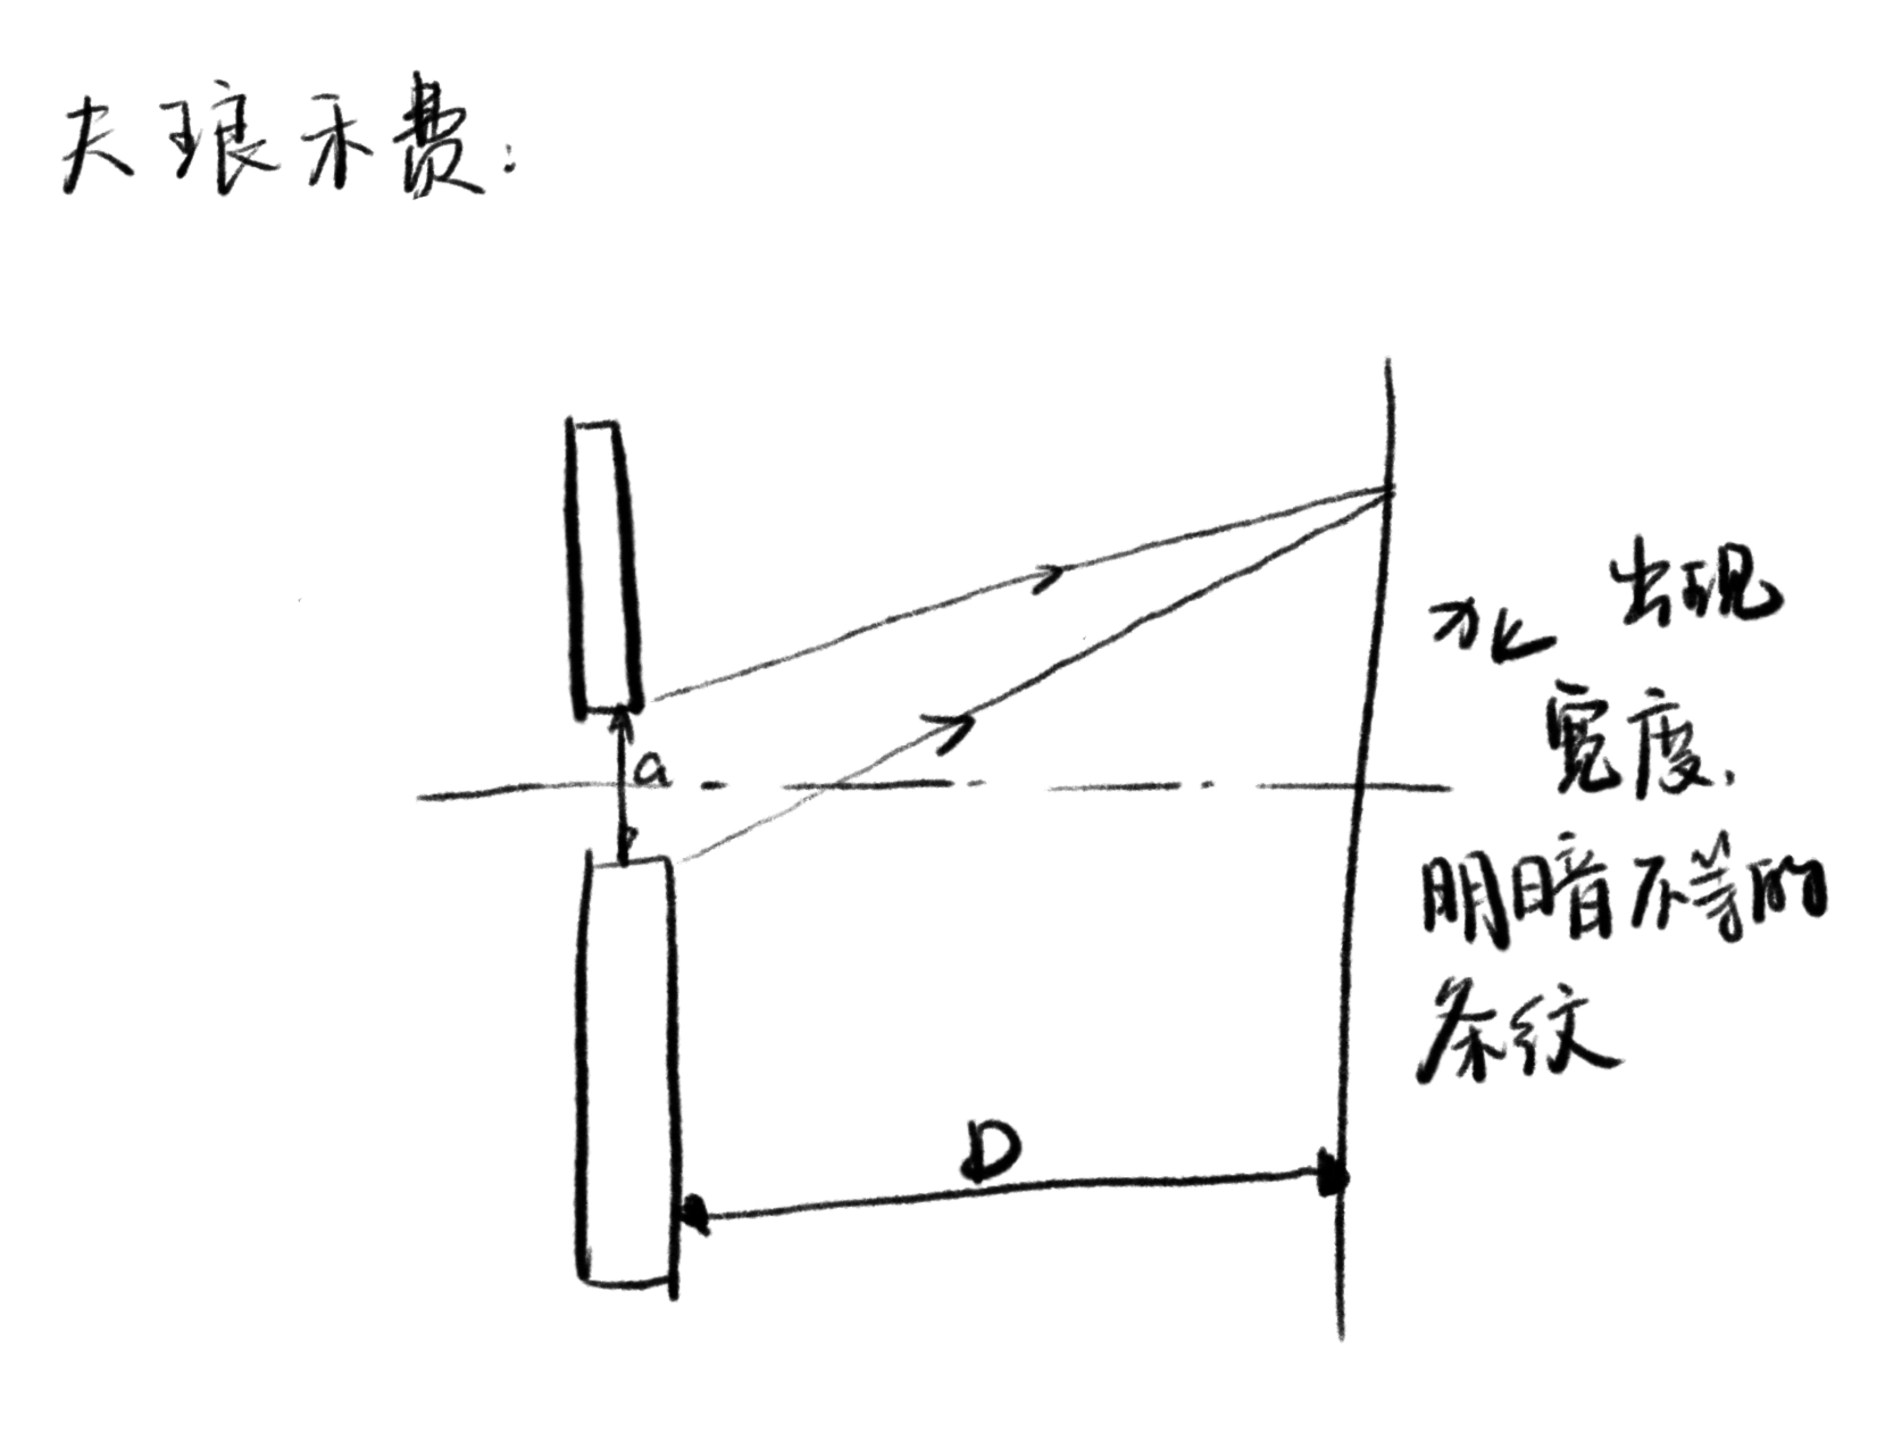
\includegraphics[width=.5\textwidth]{夫.pdf}
    \caption{夫琅禾费衍射}
\end{figure}

\paragraph{利用光栅衍射法测量激光波长}
光栅方程(主极大条件):
\[
d\sin \theta = \pm k\lambda(k = 0, \pm 1, \pm 2, \cdots)
\]
角度较小时,我们有$\sin\theta \approx \tan \theta \approx \frac{x}{D}$,即
\[
x_k = k\frac{D}{d}\lambda
\]
最后由公式\[\frac{x_1 - x_{-1}}{2} \approx \frac{D}{d}\lambda\]
可以求出激光波长
\begin{figure}[H]
    \centering
    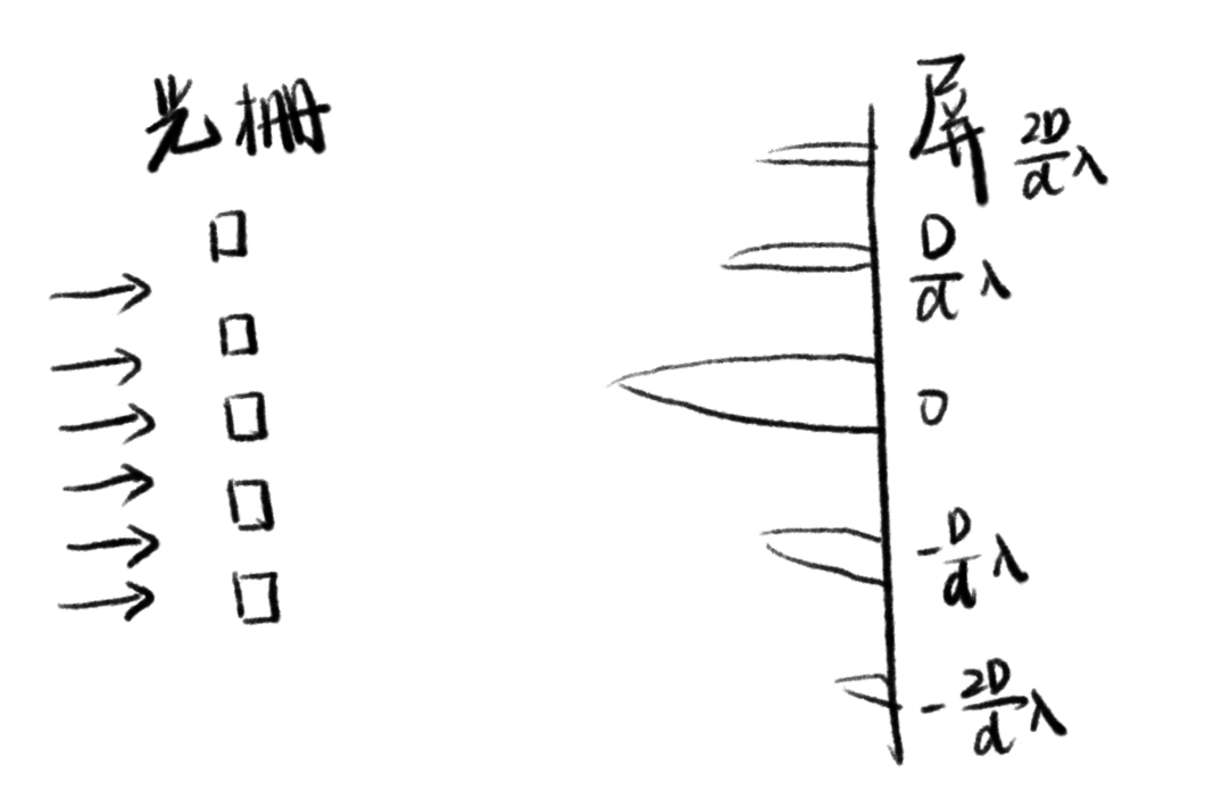
\includegraphics[width=.3\textwidth]{光栅.pdf}
    \caption{光栅衍射法测光的波长}
\end{figure}
\subsubsection{实验方法}
\begin{enumerate}
    \item \textbf{光路调节与校准:}
    调节光学导轨上的各个光学元件,确保它们的位置共轴且等高,以形成一条清晰、水平的实验光路。

    \item \textbf{观察不同孔隙的衍射图样:}
    将具有不同形状孔隙的衍射板置于光路中,定性观察并记录各自产生的夫琅禾费衍射图样的形状特征。

    \item \textbf{利用一维光栅测定激光波长:}
    使用一维光栅(已知参数为 50 条/\si{\mm})进行衍射实验。精确测量其衍射图样中正一级与负一级主极大亮纹之间的距离,然后依据光栅方程 $\frac{x_1 - x_{-1}}{2} \approx \frac{D}{d}\lambda$ 计算出所用激光的波长 $\lambda$。

    \item \textbf{研究单缝衍射的光强分布并测量缝宽:}
    观察由单缝产生的夫琅禾费衍射条纹。利用一维光强测量仪测出其光强分布。绘制出相对光强 $I/I_0$ 随位置坐标 $x$ 变化的函数图像,并根据衍射图样中暗纹的位置,计算出该单缝的精确宽度 $a$。

\end{enumerate}
\subsection{实验重点(3分)}
(简述本实验的学习重点,不超过100字。)
\begin{enumerate}
    \item \textbf{分析衍射图案:}首先要搞清楚,当光线通过不同形状的物体时,产生的衍射花样的明暗分布有什么不同和规律。
    \item \textbf{应用衍射原理进行测量:}要学会并熟练运用光的衍射,去测量一些微小量
    % \item \textbf{了解更复杂的衍射:}最后,还需要了解当光通过二维光栅时,会产生怎样的衍射特征。
\end{enumerate}
\subsection{实验难点(2分)}
(简述本实验的实现难点,不超过100字。)
\begin{enumerate}
    \item 实验开始前需要调整光学导轨,确保各光学元件等高
    % \item 读数需要小心,计算$D$的时候,接收屏位置$L_2$并非读数
    \item 转动轮毂时为了避免空程差,不能往回传,只能单向转动
    \item 测量的时候不能移动光学仪器的位置
\end{enumerate}
\begin{fullreportonly}
\section{原始数据(20分)}
(将有老师签名的“自备数据记录草稿纸”的扫描或手机拍摄图粘贴在下方,完整保留姓名,学号,教师签字和日期。)

见\cref{data}
\section{结果与分析(60分)}
\subsection{数据处理与结果(30分)}
\subsubsection{利用光栅衍射法测量光的波长}
% Please add the following required packages to your document preamble:
% \usepackage{graphicx}
\begin{table}[H]
\centering
\caption{利用光栅衍射法测量光的波长数据记录表}
\label{tab:lambda}
% \resizebox{\textwidth}{!}{%
\begin{tabular}{|ll|ll|l|}
\hline
\multicolumn{1}{|l|}{序号} & $x_{+1}(\si{\mm})$ & \multicolumn{1}{l|}{$x_{-1}(\si{\mm})$} & $x_{+1} - x_{-1}(\si{\mm})$ & $\lambda(\si{\mm})$                        \\ \hline
\multicolumn{1}{|l|}{1} & 73.745 & \multicolumn{1}{l|}{31.445} & 42.300 & 631.3 \\ \hline
\multicolumn{1}{|l|}{2} & 73.151 & \multicolumn{1}{l|}{31.145} & 43.006 & 641.9 \\ \hline
\multicolumn{1}{|l|}{3} & 73.725 & \multicolumn{1}{l|}{31.127} & 42.598 & 635.8 \\ \hline
\multicolumn{1}{|l|}{4} & 73.640 & \multicolumn{1}{l|}{31.019} & 42.621 & 636.1 \\ \hline
\multicolumn{1}{|l|}{5} & 73.720 & \multicolumn{1}{l|}{31.132} & 42.588 & 635.6 \\ \hline
\multicolumn{1}{|l|}{6} & 73.607 & \multicolumn{1}{l|}{30.901} & 42.706 & 637.4 \\ \hline
\multicolumn{2}{|c|}{衍射屏位置 \SI{70.00}{\cm}}   & \multicolumn{2}{c|}{接收屏位置 \SI{30.00}{\cm}}                            & \multicolumn{1}{c|}{发射器位置\SI{117.00}{\cm}} \\ \hline
\end{tabular}%
% }
\end{table}
\[
\overline{\Delta x} = \overline{x_{+1} - x_{-1}} = \frac{42.300 + 43.006 + \cdots + 42.588 + 42.706}{6} = 42.636 \si{\mm}
\]
根据$\pm \lambda = (a + b)\sin \theta$, $\sin \theta \approx \theta \approx \tan \theta = \frac{\Delta x}{2\Delta L}$. 其中$a + b = \SI{0.02}{\mm}$,$\Delta L = \SI{670.0}{\mm}$,得出
\[
\lambda = \frac{(a + b)\Delta x}{2\Delta L} = \frac{\SI{0.02}{\mm} \times \SI{42.636}{\mm}}{2 \times \SI{670.0}{\mm}} = \SI{636.4}{\nm}
\]
不确定度计算:
\[
u_A(\bar{x}) = \sqrt{\frac{\sum{(x_i - \bar{x})^2}}{n(n-1)}} = \SI{0.093}{\mm}
\]
螺旋测微计的不确定度$u_B = \SI{0.004}{\mm}$

则合成不确定度:
\[u_{\bar{\Delta x}} = \sqrt{u_A^2 + u_B^2} = \sqrt{(0.093)^2 + (0.004)^2} \approx \SI{0.0931}{\mm}\]

$u_L = \frac{\SI{1}{\milli \meter}}{\sqrt{3}}$,则:
\[
\frac{u_\lambda}{\lambda} = \sqrt{\frac{u_{\bar{\Delta x}}}{\bar{\Delta x}}^2 + \frac{u_L}{L}^2} = 0.23\%
\]
因此
\[
u_\lambda = 1.5nm
\]
即
\[
\lambda = \SI{636.4(1.5)}{\nano\meter}
\]
\subsubsection{利用单缝衍射测出狭缝宽度}
\begin{table}[H]
\centering
\caption{利用单缝衍射测狭缝宽度数据记录表}
\label{tab:a}
% \resizebox{\textwidth}{!}{%
\begin{tabular}{|ll|ll|l|}
\hline
\multicolumn{1}{|l|}{序号} & $x_{+1}(\si{\mm})$ & \multicolumn{1}{l|}{$x_{-1}(\si{\mm})$} & $x_{+1} - x_{-1}(\si{\mm})$ & $a(\si{\micro \meter})$                    \\ \hline
\multicolumn{1}{|l|}{1} & 60.162 & \multicolumn{1}{l|}{42.915} & 17.247 & 70.6 \\ \hline
\multicolumn{1}{|l|}{2} & 59.680 & \multicolumn{1}{l|}{43.005} & 16.676 & 73.0 \\ \hline
\multicolumn{1}{|l|}{3} & 59.460 & \multicolumn{1}{l|}{42.540} & 16.920 & 72.0 \\ \hline
\multicolumn{1}{|l|}{4} & 59.330 & \multicolumn{1}{l|}{42.330} & 17.000 & 71.6 \\ \hline
\multicolumn{1}{|l|}{5} & 59.671 & \multicolumn{1}{l|}{42.112} & 17.559 & 69.3 \\ \hline
\multicolumn{1}{|l|}{6} & 59.955 & \multicolumn{1}{l|}{42.055} & 17.405 & 69.9 \\ \hline
\multicolumn{2}{|c|}{衍射屏位置 \SI{70.00}{\cm}}   & \multicolumn{2}{c|}{接收屏位置 \SI{30.00}{\cm}}                            & \multicolumn{1}{c|}{发射器位置\SI{117.00}{\cm}} \\ \hline
\end{tabular}%
% }
\end{table}
由单缝衍射一级亮纹的位置$\sin \theta = \pm 1.43 \frac{\lambda}{a}$,且$\sin \theta \approx \theta \approx \tan \theta = \frac{\Delta x}{2\Delta L}$,其中$\Delta L = \SI{670.0}{\mm}$,得出
\[
a = \frac{1.43 \cdot 2L\lambda}{\Delta x}
\]
\[
\overline{\Delta x} = \frac{17.247 + 16.676 + 16.920 + 17.000 + 17.559 + 17.405}{6} = 17.134 \si{\mm}
\]
可得
\[a = \frac{1.43 \cdot 2 \cdot 670.0 \cdot 0.6364}{17.134} = \SI{71.2}{\micro \meter}\]
不确定度:
\[
\frac{u_a}{a} = \sqrt{\left(\frac{u_\lambda}{\lambda}\right)^2 + \left(\frac{u_{\Delta x}}{\Delta x}\right)^2 + \left(\frac{u_{L}}{L}\right)^2}
\]
其中$\Delta x$的A类不确定度$u_A = \sqrt{\frac{\sum{(x_i - \bar{x})^2}}{n(n-1)}} = \SI{0.134}{\mm}$,B类不确定度$u_B = \SI{0.004}{\mm}$,则合成不确定度$u_{\Delta x} = \sqrt{u_A^2 + u_B^2} = \SI{0.134}{\mm}$

则合成不确定度
\[
\frac{u_a}{a} = \sqrt{\left(\frac{u_\lambda}{\lambda}\right)^2 + \left(\frac{u_{\Delta x}}{\Delta x}\right)^2 + \left(\frac{u_{L}}{L}\right)^2} = 0.402\%
\]
\[
u_a = a * \frac{u_a}{a} = \SI{0.3}{\micro \meter}
\]
则最终结果狭缝宽度$a$:
\[
a = \SI{71.2(0.3)}{\micro \meter}
\]
\subsubsection{绘制单缝衍射中光强分布}
从-2级暗纹到+2级暗纹中,每\SI{0.400}{\mm}测量一次光强,输入至\textrm{Origin}中绘制出光强(光电流)随位置坐标$x$变化的函数图像,如\cref{fig:intensity}所示。
\begin{figure}[H]
    \centering
    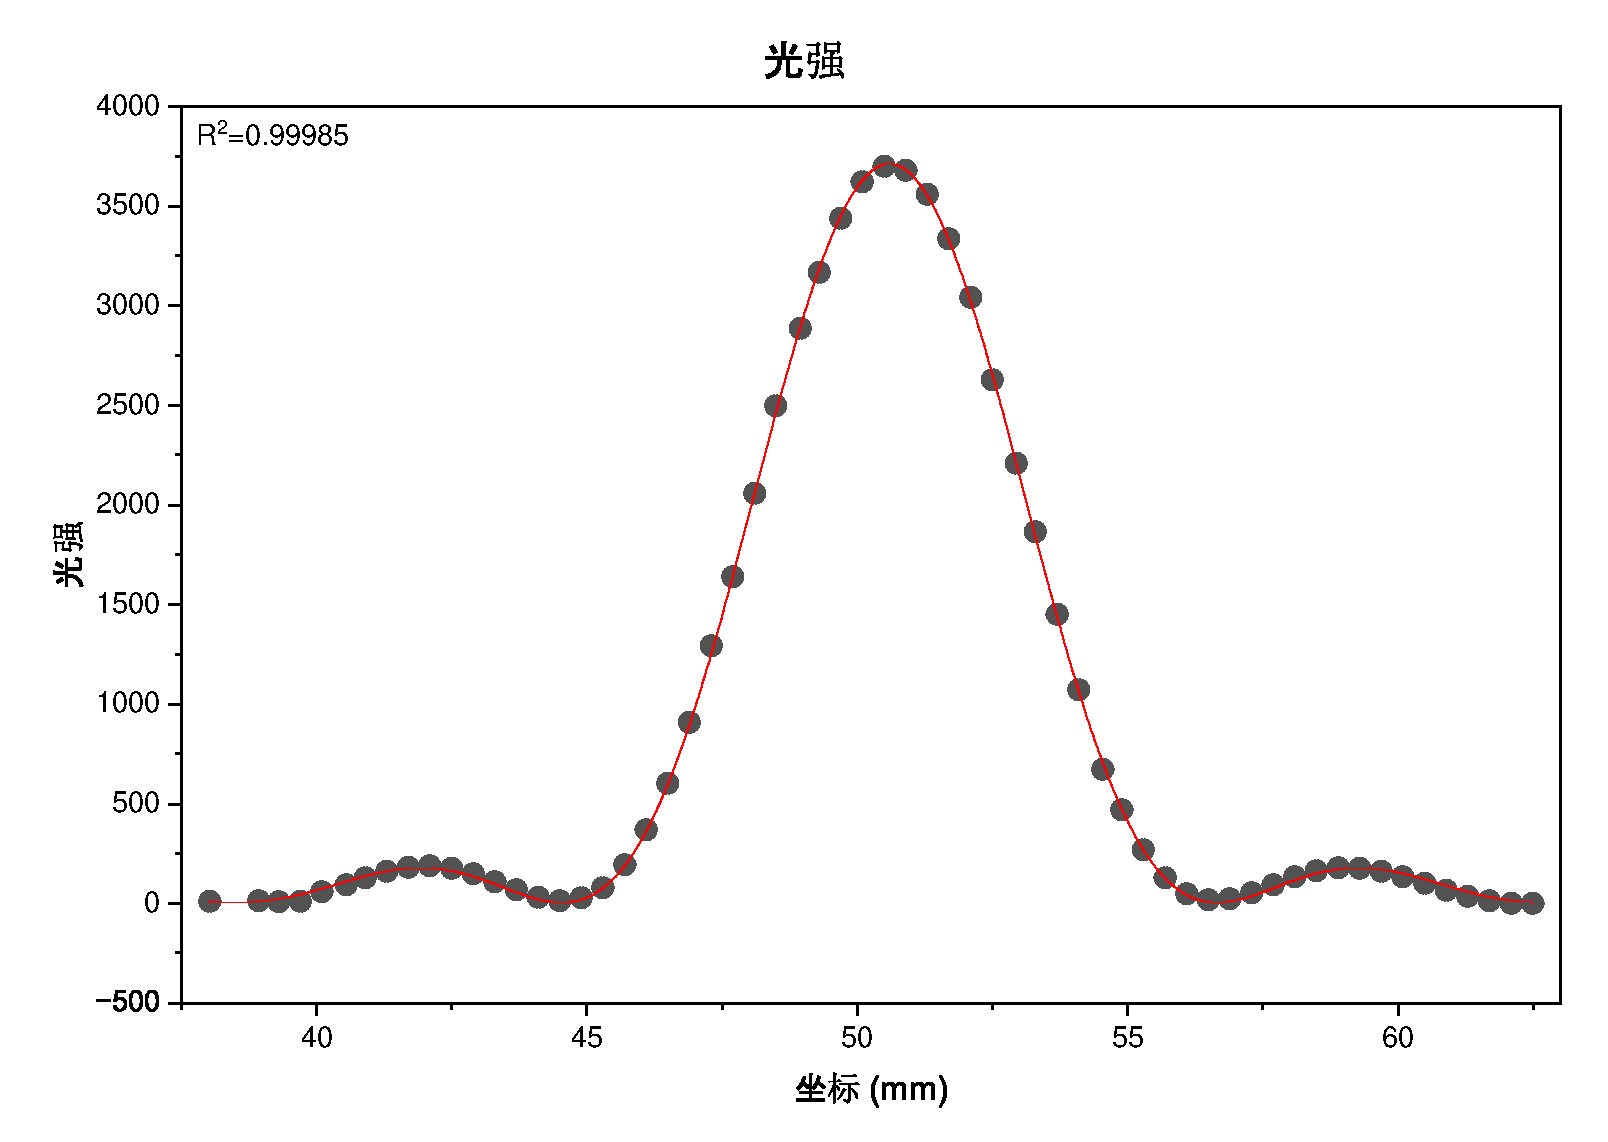
\includegraphics[width=.7\textwidth]{intensity.pdf}
    \caption{单缝衍射中光强分布图像}
    \label{fig:intensity}
\end{figure}
因为光强符合
\[
I(x) = I_0\left[\frac{\sin \beta}{\beta}\right]^2
\]
因此使用函数
\[
y = y_0 + A\cdot\left(\frac{\sin(w \cdot (x - x_c))}{w \cdot (x - x_c)}\right)^2
\]
进行拟合,其中$y_0$为基准偏移量,$A$为振幅,$w$为宽度调节参数,$x_c$为中心位置偏移量。拟合具体结果见\cref{res}。
\subsubsection{验证光强公式}
测得0级亮纹的最大光强是$I_0 = 3622.8$, 一级亮纹的亮度是$I_1 = 182.7$
\[
\frac{182.7}{3622.8} = 5.04\% \approx 4.7\%
\]
\subsection{误差分析(20分)}
(运用测量误差、相对误差或不确定度等分析实验结果,写出完整的结果表达式,并分析误差原因。)
\subsubsection{利用光栅衍射法测量光的波长}
\paragraph{相对误差}
\[E_\lambda = \frac{\left|\lambda_\text{理论} - \lambda_\text{实际}\right|}{\lambda_\text{理论}} = \frac{636.4 - 635}{635} = 0.22\%\]
\[E_a = \frac{\left|a_\text{理论} - a_\text{实际}\right|}{a_\text{理论}} = \frac{80.0 - 71.2}{80} = 11\%\]
可见,测量光的波长相对误差很小,实验较为成功;但是测量狭缝时与理论值产生了较大的偏差。
\paragraph{误差来源分析}
\begin{enumerate}
    \item 实验中,各光学仪器难以调整至完全等高,可能对结果有所影响
    \item 实验中难以真正找到单缝或者光栅衍射时的极大值,对+1级亮纹到-1级亮纹之间的距离测量有所影响
    \item 狭缝可能并非完全理想的单缝,可能存在一定的加工误差,导致测量值与理论值不能很好吻合
    \item 读数$L$, $x$时都需要估读,可能引入误差
\end{enumerate}
\subsection{实验探讨(10分)}
(对实验内容、现象和过程的小结,不超过100字。)

这是在本学期我做完分光计的调整和测量棱镜顶角之后的第二个实验,由于要测量很多组数据,很好的锻炼了我的耐心,而且通过拟合这些数据,让我对
使用Origin等数据处理分析软件有了更深的了解。同时不确定度的计算较为复杂,让我对不确定度这一概念及其计算方法有了更深的了解。
\section{思考题(10分)}
(解答教材或讲义或老师布置的思考题,请先写题干,再作答。)
\subsection{单缝衍射两侧光强不是严格对称的原因是什么?}
最主要的原因是激光光斑没有精确地对准狭缝的中心位置,或者激光没有垂直打入狭缝,而是与狭缝产生了一定角度,导致两侧的光强分布不对称。但也有可能是狭缝本身制作不够精细,导致狭缝两侧的边缘不够平直,从而影响了衍射图样的对称性。
\subsection{狭缝太宽或太窄会发生什么情况,为什么?}
\paragraph{太宽:}
太宽的时候,可能明纹和暗纹都无法区分,明暗条纹被压缩,变得很细很密,导致无法测量。
当狭缝足够宽的时候,光线几乎不发生衍射现象,光线基本上是直线传播的,接收屏上看到的只是一个均匀的亮斑(狭缝的影子),而没有明显的衍射条纹。
\paragraph{太窄:}
太窄可能会导致光强过弱,无法看到清晰的衍射条纹,导致难以测量,无法得出正确的结论。当狭缝足够小的时候,可能没有光线能够满足单缝衍射暗纹的方程,即中央的明纹扩散至整个接收屏。
\subsection{光栅衍射时会发生缺级现象,为什么?}
\paragraph{定性分析:}
光栅衍射是光在多个单缝中衍射之后,再进行干涉的结果。如果干涉中的主极大位置恰好位于衍射的暗纹区域,那么该级主极大就会消失,形成缺级现象。
\paragraph{定量分析:}
多缝干涉是由由光栅上所有狭缝之间的光程差决定,满足\[
d\sin\theta = k\lambda (k = 0, \pm 1, \pm 2, \cdots)
\]
其中$d$为光栅常数。

而单缝衍射的光强是由每个单缝的宽度决定,满足\[
a\sin\theta = m\lambda (m = 0, \pm 1, \pm 2, \cdots)
\]
其中$a$为狭缝宽度。
如果当一个$\theta$满足既在干涉的极大值上,又是在衍射的极小值上时,就会发生缺级现象。即当存在$k$和$m$使得
\[
\frac{d}{a} = \frac{k}{m}
\]
时,就会发生缺级现象。

在PPT所示的例子中,$\sin\theta = 4\frac{\lambda}{d}$处发生缺级现象,就是因为光栅常数$d$和狭缝宽度$a$满足$\frac{d}{a} = 4$,那么第一级衍射暗条纹就会落在第四级干涉极大值上,导致第四级缺级。
同理,第八,十二级也会发生缺级现象。
\subsection{在衍射的碍物为圆屏时,无论圆屏尺度有多大(在能够观察到衍射图样的范围内),衍射图样的中心总会有一个亮斑,请解释这个现象发生的原因。}
当一束光照射到一个不透明的圆屏时,圆屏会挡住波前的中心部分。但是,圆屏边缘的波前没有被挡住。
根据惠更斯原理,圆屏边缘上的每一个点都成为了一个新的子波源,向各个方向发光。
现在我们只考虑阴影区域最正中心的那个点(我们称之为 $P$)。
由于圆屏是完美对称的圆形,圆屏边缘上的所有点到阴影中心点 $P$ 的几何距离是完全相等的。
因为所有来自圆屏边缘的子波源到达 $P$ 点的路程都相等,所以它们到达 $P$ 点时同相。当所有波同相叠加时,它们会发生相长干涉,导致光强在这一点被大大加强,从而形成一个亮斑。
而对于阴影区域中非中心的任意一点,它到圆屏边缘不同点的距离是不相等的。这导致来自边缘的波到达该点时具有不同的相位,它们会相互抵消,因此这些区域不会出现亮斑。
\end{fullreportonly}
\insertnotes
\begin{fullreportonly}
    \clearpage
\appendix
\section{原始数据}\label{data}
\section{拟合的结果}\label{res}
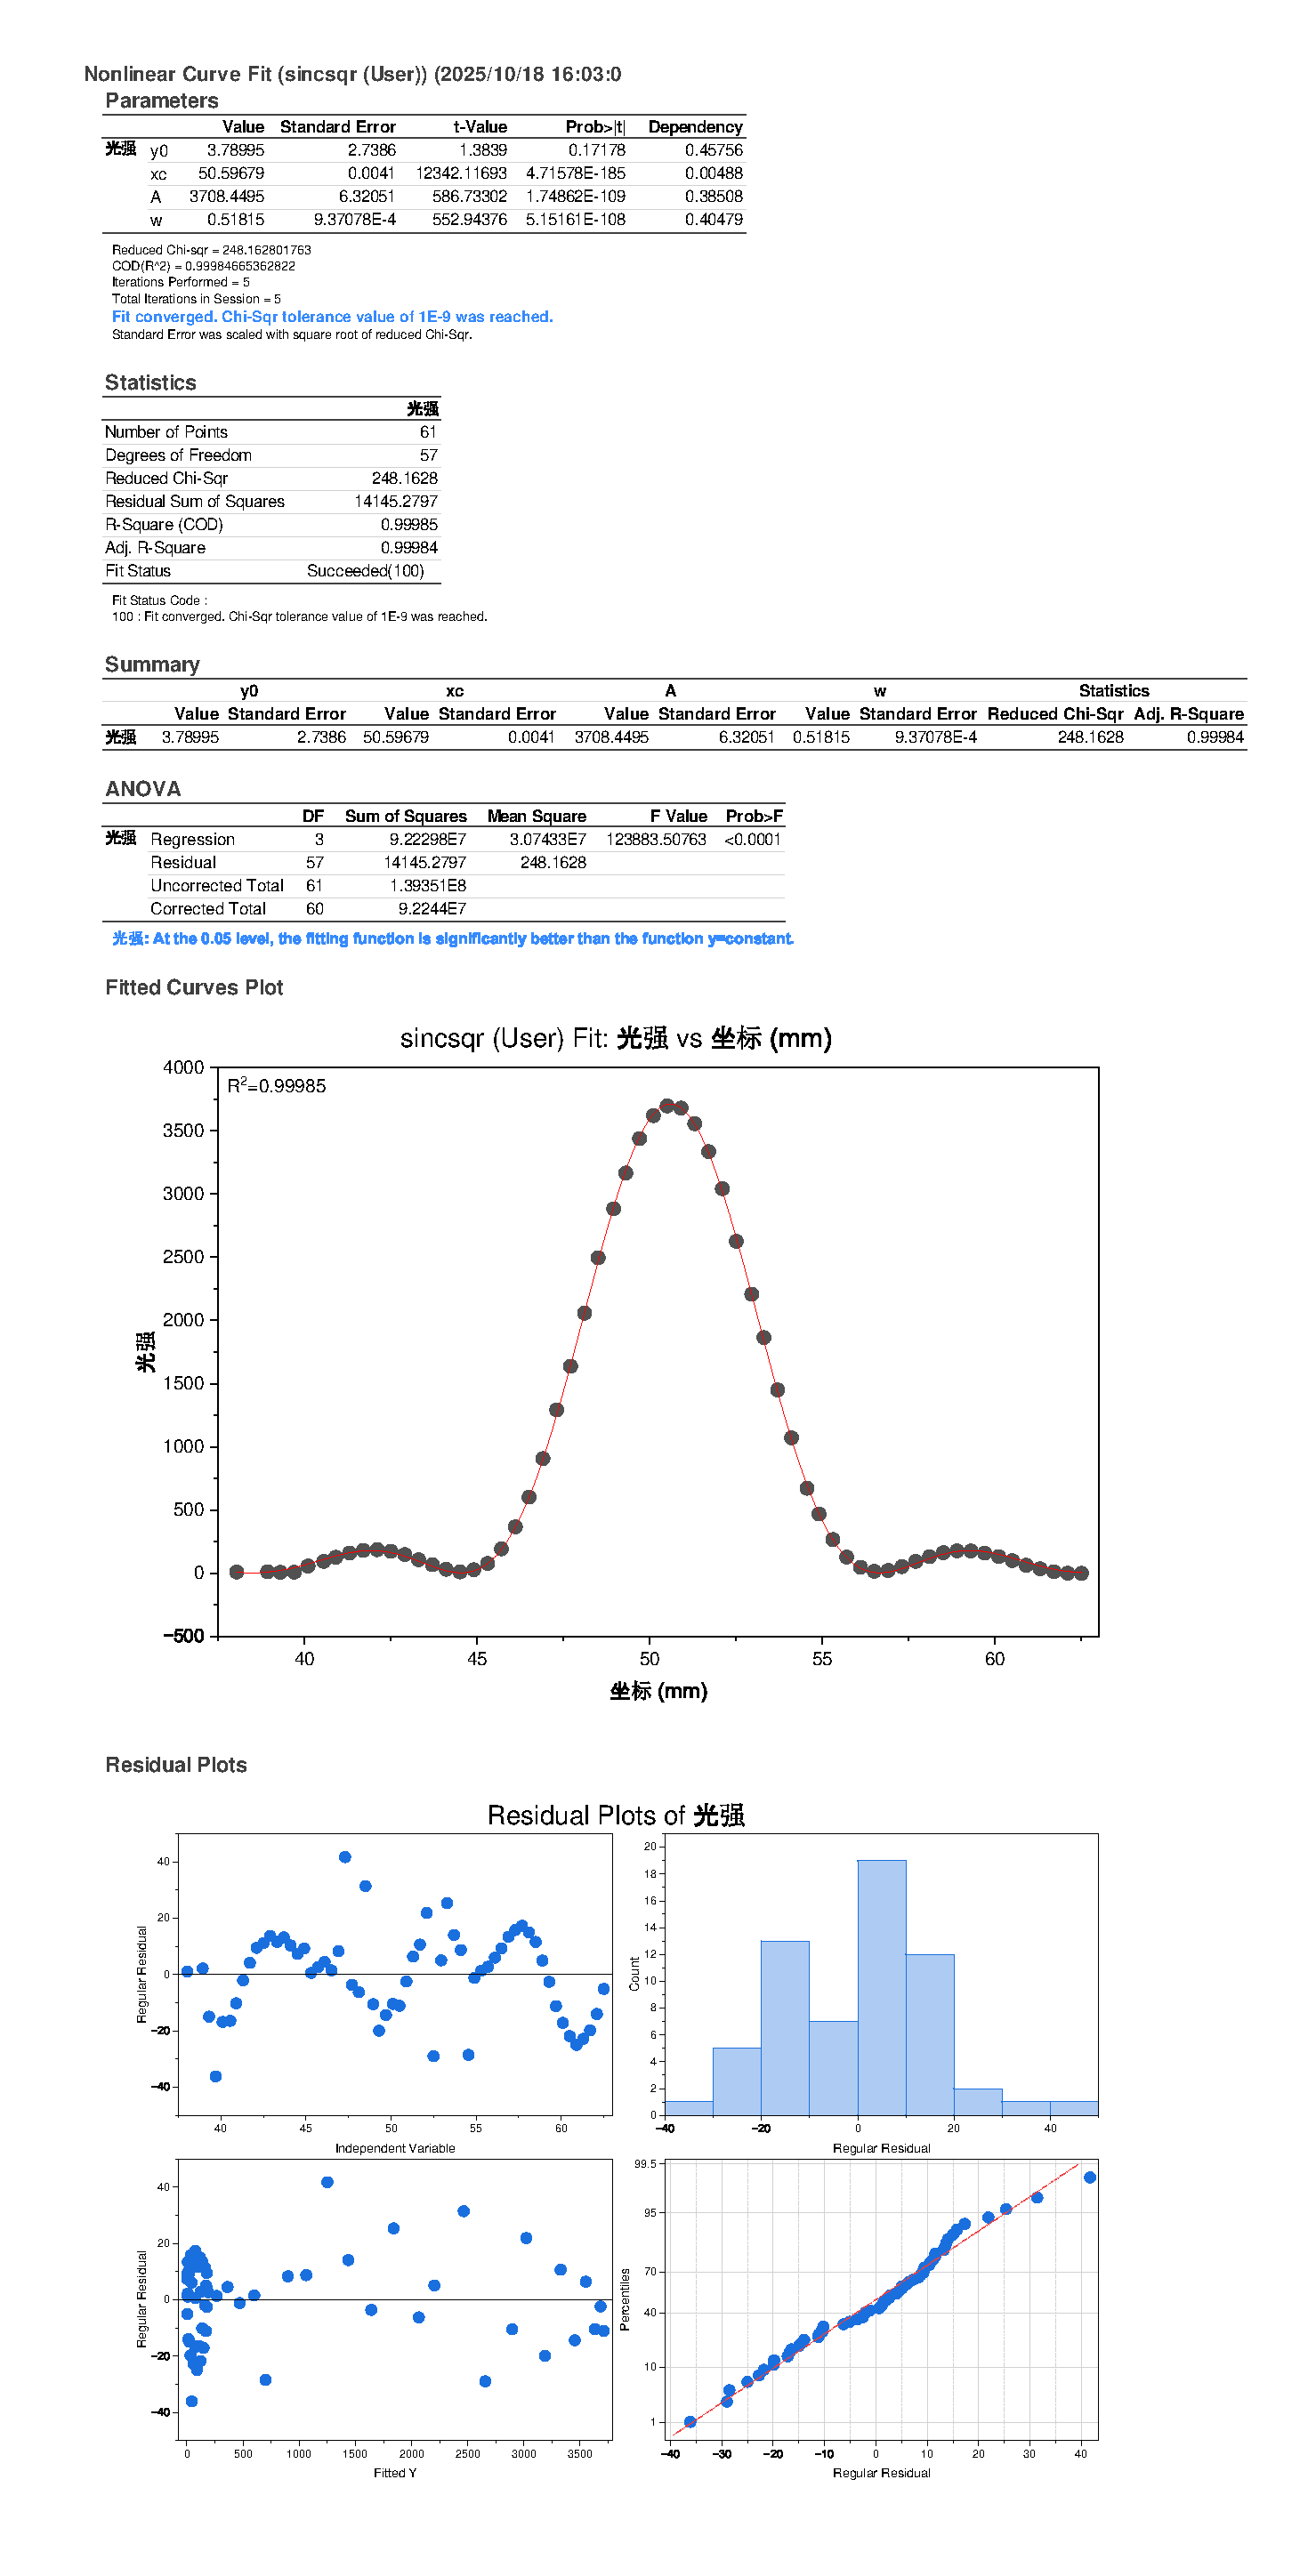
\includepdf[page=1]{./figures/fit.pdf}
\end{fullreportonly}
\end{document}